\section{Results}
\label{sec:svbrdf:results}

\textbf{Only a small subset of our results fits into the paper. Please see our supplemental material and video for more results.}

\paragraph{Test data.}
For synthetic tests, we use several examples from the test set of Deschaintre \cite{deschaintre2018single}, as well as some from the Adobe Stock dataset \cite{li2018materials}. This gives a total of 30 synthetic results.
For our real results, we use a hand-held mobile phone to capture images with flash, resulting in a collocated camera and point light illumination.
Similar to previous work \cite{hui2017reflectance,deschaintre2019flexible}, we use a paper frame to register the multiple images.
We add markers to the frame to improve camera pose estimation.
Using this process, we capture 40 physical samples with nine images per material, roughly covering the sample with $3 \times 3$ specular highlights. 
Unless otherwise specified, all our results use seven images for inverse-rendering optimizations and the remaining two (under novel lighting) for evaluating the results.

\paragraph{Inverse-rendering performance.}
Our optimization takes about 2 minutes to complete 2000 iterations on a Titan RTX GPU. In many cases, the results converge after ~500 iterations, but we use 2000 everywhere for simplicity.

\begin{figure}[!ht]
	\centering
	\setlength{\resLen}{0.85in}
	\setlength{\raiseLen}{.3in}
	\addtolength{\tabcolsep}{-4pt}
	\begin{tabular}{ccccc}
		& SVBRDF maps & Optimization & \multicolumn{2}{c}{Novel views}
		\\
		\raisebox{\raiseLen}{\rotatebox[origin=c]{90}{GT}} &
		\includegraphics[height=\resLen]{svbrdf/results/fake/fake_022/ref/tex.jpg} &
		
\includegraphics[height=\resLen]{svbrdf/results/fake/fake_022/ref/00.jpg} &
		\includegraphics[height=\resLen]{svbrdf/results/fake/fake_022/ref/07.jpg} &
		\includegraphics[height=\resLen]{svbrdf/results/fake/fake_022/ref/08.jpg}
		\\
		\raisebox{\raiseLen}{\rotatebox[origin=c]{90}{Ours}} &
		\includegraphics[height=\resLen]{svbrdf/results/fake/fake_022/ours+/tex.jpg} &
		
\includegraphics[height=\resLen]{svbrdf/results/fake/fake_022/ours+/00.jpg} &
		\includegraphics[height=\resLen]{svbrdf/results/fake/fake_022/ours+/07.jpg} &
		\includegraphics[height=\resLen]{svbrdf/results/fake/fake_022/ours+/08.jpg}
		\\
		\raisebox{\raiseLen}{\rotatebox[origin=c]{90}{GT}} &
		\includegraphics[height=\resLen]{svbrdf/results/fake/fake_039/ref/tex.jpg} &
		
\includegraphics[height=\resLen]{svbrdf/results/fake/fake_039/ref/00.jpg} &
		\includegraphics[height=\resLen]{svbrdf/results/fake/fake_039/ref/07.jpg} &
		\includegraphics[height=\resLen]{svbrdf/results/fake/fake_039/ref/08.jpg}
		\\
		\raisebox{\raiseLen}{\rotatebox[origin=c]{90}{Ours}} &
		\includegraphics[height=\resLen]{svbrdf/results/fake/fake_039/ours+/tex.jpg} &
		
\includegraphics[height=\resLen]{svbrdf/results/fake/fake_039/ours+/00.jpg} &
		\includegraphics[height=\resLen]{svbrdf/results/fake/fake_039/ours+/07.jpg} &
		\includegraphics[height=\resLen]{svbrdf/results/fake/fake_039/ours+/08.jpg}
	\end{tabular}
	\caption[SVBRDF reconstruction on synthetic data]{\label{fig:svbrdf:synthetic}
		\textbf{SVBRDF reconstruction on synthetic data.} We demonstrate results on synthetic SVBRDFs, one from \cite{deschaintre2019flexible} (top) and one from the Adobe Stock Material dataset (bottom). We are able to accurately reconstruct these materials from 7 input images (one input shown). Many more synthetic results are available in supplementary materials.
	}
\end{figure}

\paragraph{Testing on synthetic data.}
Figure \ref{fig:svbrdf:synthetic} contains two synthetic results using our method, showing a close match both in maps and in novel view renderings. For more results, please refer to supplemental materials. We note that all methods perform better on synthetic data than on real data, possibly because of the exact BRDF model match and perfect calibration, and also
because the synthetic test set, while distinct from the training set, is relatively similar in style.

\begin{figure}[h!]
    \centering
    \setlength{\resLen}{.43in}
    \setlength{\raiseLen}{.2in}
    \addtolength{\tabcolsep}{-5pt}
    \scriptsize
    \begin{tabular}{rlrccc@{\hspace{2\tabcolsep}}lrccc}
        & \multicolumn{2}{c}{SVBRDF maps} & Opt. & \multicolumn{2}{c}{Novel views}
        & \multicolumn{2}{c}{SVBRDF maps} & Opt. & \multicolumn{2}{c}{Novel views}
        \\[1pt]
        &
        \raisebox{3pt}{\textit{~~wall-plaster-white}} & \raisebox{0.40\resLen}{\rotatebox[origin=c]{90}{GT}}&
        
\includegraphics[height=\resLen]{svbrdf/results/main/real_wall-plaster-white/ref/00.jpg} &
        \includegraphics[height=\resLen]{svbrdf/results/main/real_wall-plaster-white/ref/07.jpg} &
        \includegraphics[height=\resLen]{svbrdf/results/main/real_wall-plaster-white/ref/08.jpg} &
        \raisebox{3pt}{\textit{~~plastic-red-carton}} & \raisebox{0.40\resLen}{\rotatebox[origin=c]{90}{GT}}&
        
\includegraphics[height=\resLen]{svbrdf/results/main/real_plastic-red-carton/ref/00.jpg} &
        \includegraphics[height=\resLen]{svbrdf/results/main/real_plastic-red-carton/ref/07.jpg} &
        \includegraphics[height=\resLen]{svbrdf/results/main/real_plastic-red-carton/ref/08.jpg}
        \\
        \raisebox{\raiseLen}{\rotatebox[origin=c]{90}{Ours}} &
        \multicolumn{2}{c}{\includegraphics[height=\resLen]{svbrdf/results/main/real_wall-plaster-white/ours+/tex.jpg}} &
        
\includegraphics[height=\resLen]{svbrdf/results/main/real_wall-plaster-white/ours+/00.jpg} &
        \includegraphics[height=\resLen]{svbrdf/results/main/real_wall-plaster-white/ours+/07.jpg} &
        \includegraphics[height=\resLen]{svbrdf/results/main/real_wall-plaster-white/ours+/08.jpg} &
        \multicolumn{2}{c}{\includegraphics[height=\resLen]{svbrdf/results/main/real_plastic-red-carton/ours+/tex.jpg}} &
        
\includegraphics[height=\resLen]{svbrdf/results/main/real_plastic-red-carton/ours+/00.jpg} &
        \includegraphics[height=\resLen]{svbrdf/results/main/real_plastic-red-carton/ours+/07.jpg} &
        \includegraphics[height=\resLen]{svbrdf/results/main/real_plastic-red-carton/ours+/08.jpg}
        \\
        \raisebox{\raiseLen}{\rotatebox[origin=c]{90}{[Gao19]+}} &
        \multicolumn{2}{c}{\includegraphics[height=\resLen]{svbrdf/results/main/real_wall-plaster-white/msra+_egsr/tex.jpg}} &
        
\includegraphics[height=\resLen]{svbrdf/results/main/real_wall-plaster-white/msra+_egsr/00.jpg} &
        \includegraphics[height=\resLen]{svbrdf/results/main/real_wall-plaster-white/msra+_egsr/07.jpg} &
        \includegraphics[height=\resLen]{svbrdf/results/main/real_wall-plaster-white/msra+_egsr/08.jpg} &
        \multicolumn{2}{c}{\includegraphics[height=\resLen]{svbrdf/results/main/real_plastic-red-carton/msra+_egsr/tex.jpg}} &
        
\includegraphics[height=\resLen]{svbrdf/results/main/real_plastic-red-carton/msra+_egsr/00.jpg} &
        \includegraphics[height=\resLen]{svbrdf/results/main/real_plastic-red-carton/msra+_egsr/07.jpg} &
        \includegraphics[height=\resLen]{svbrdf/results/main/real_plastic-red-carton/msra+_egsr/08.jpg}
        \\[1pt]
        &
        \raisebox{3pt}{\textit{~~leather-blue}} & \raisebox{0.40\resLen}{\rotatebox[origin=c]{90}{GT}}&
        
\includegraphics[height=\resLen]{svbrdf/results/main/real_leather-blue/ref/00.jpg} &
        \includegraphics[height=\resLen]{svbrdf/results/main/real_leather-blue/ref/07.jpg} &
        \includegraphics[height=\resLen]{svbrdf/results/main/real_leather-blue/ref/08.jpg} &
        \raisebox{3pt}{\textit{~~bathroomtile2}} & \raisebox{0.40\resLen}{\rotatebox[origin=c]{90}{GT}}&
        
\includegraphics[height=\resLen]{svbrdf/results/main/real_bathroomtile2/ref/00.jpg} &
        \includegraphics[height=\resLen]{svbrdf/results/main/real_bathroomtile2/ref/07.jpg} &
        \includegraphics[height=\resLen]{svbrdf/results/main/real_bathroomtile2/ref/08.jpg}
        \\
        \raisebox{\raiseLen}{\rotatebox[origin=c]{90}{Ours}} &
        \multicolumn{2}{c}{\includegraphics[height=\resLen]{svbrdf/results/main/real_leather-blue/ours+/tex.jpg}} &
        
\includegraphics[height=\resLen]{svbrdf/results/main/real_leather-blue/ours+/00.jpg} &
        \includegraphics[height=\resLen]{svbrdf/results/main/real_leather-blue/ours+/07.jpg} &
        \includegraphics[height=\resLen]{svbrdf/results/main/real_leather-blue/ours+/08.jpg} &
        \multicolumn{2}{c}{\includegraphics[height=\resLen]{svbrdf/results/main/real_bathroomtile2/ours+/tex.jpg}} &
        
\includegraphics[height=\resLen]{svbrdf/results/main/real_bathroomtile2/ours+/00.jpg} &
        \includegraphics[height=\resLen]{svbrdf/results/main/real_bathroomtile2/ours+/07.jpg} &
        \includegraphics[height=\resLen]{svbrdf/results/main/real_bathroomtile2/ours+/08.jpg}
        \\
        \raisebox{\raiseLen}{\rotatebox[origin=c]{90}{[Gao19]+}} &
        \multicolumn{2}{c}{\includegraphics[height=\resLen]{svbrdf/results/main/real_leather-blue/msra+_egsr/tex.jpg}} &
        \includegraphics[height=\resLen]{svbrdf/results/main/real_leather-blue/msra+_egsr/00.jpg} &
        \includegraphics[height=\resLen]{svbrdf/results/main/real_leather-blue/msra+_egsr/07.jpg} &
        \includegraphics[height=\resLen]{svbrdf/results/main/real_leather-blue/msra+_egsr/08.jpg} &
        \multicolumn{2}{c}{\includegraphics[height=\resLen]{svbrdf/results/main/real_bathroomtile2/msra+_egsr/tex.jpg}} &
        \includegraphics[height=\resLen]{svbrdf/results/main/real_bathroomtile2/msra+_egsr/00.jpg} &
        \includegraphics[height=\resLen]{svbrdf/results/main/real_bathroomtile2/msra+_egsr/07.jpg} &
        \includegraphics[height=\resLen]{svbrdf/results/main/real_bathroomtile2/msra+_egsr/08.jpg}
        \\[1pt]
        &
        \raisebox{3pt}{\textit{~~wood-walnut}} & \raisebox{0.40\resLen}{\rotatebox[origin=c]{90}{GT}}&
        \includegraphics[height=\resLen]{svbrdf/results/main/real_wood-walnut/ref/00.jpg} &
        \includegraphics[height=\resLen]{svbrdf/results/main/real_wood-walnut/ref/07.jpg} &
        \includegraphics[height=\resLen]{svbrdf/results/main/real_wood-walnut/ref/08.jpg} &
        \raisebox{3pt}{\textit{~~wood-tile}} & \raisebox{0.40\resLen}{\rotatebox[origin=c]{90}{GT}}&
        \includegraphics[height=\resLen]{svbrdf/results/main/real_wood-tile/ref/00.jpg} &
        \includegraphics[height=\resLen]{svbrdf/results/main/real_wood-tile/ref/07.jpg} &
        \includegraphics[height=\resLen]{svbrdf/results/main/real_wood-tile/ref/08.jpg}
        \\
        \raisebox{\raiseLen}{\rotatebox[origin=c]{90}{Ours}} &
        \multicolumn{2}{c}{\includegraphics[height=\resLen]{svbrdf/results/main/real_wood-walnut/ours+/tex.jpg}} &
        \includegraphics[height=\resLen]{svbrdf/results/main/real_wood-walnut/ours+/00.jpg} &
        \includegraphics[height=\resLen]{svbrdf/results/main/real_wood-walnut/ours+/07.jpg} &
        \includegraphics[height=\resLen]{svbrdf/results/main/real_wood-walnut/ours+/08.jpg} &
        \multicolumn{2}{c}{\includegraphics[height=\resLen]{svbrdf/results/main/real_wood-tile/ours+/tex.jpg}} &
        \includegraphics[height=\resLen]{svbrdf/results/main/real_wood-tile/ours+/00.jpg} &
        \includegraphics[height=\resLen]{svbrdf/results/main/real_wood-tile/ours+/07.jpg} &
        \includegraphics[height=\resLen]{svbrdf/results/main/real_wood-tile/ours+/08.jpg}
        \\
        \raisebox{\raiseLen}{\rotatebox[origin=c]{90}{[Gao19]+}} &
        \multicolumn{2}{c}{\includegraphics[height=\resLen]{svbrdf/results/main/real_wood-walnut/msra+_egsr/tex.jpg}} &
        \includegraphics[height=\resLen]{svbrdf/results/main/real_wood-walnut/msra+_egsr/00.jpg} &
        \includegraphics[height=\resLen]{svbrdf/results/main/real_wood-walnut/msra+_egsr/07.jpg} &
        \includegraphics[height=\resLen]{svbrdf/results/main/real_wood-walnut/msra+_egsr/08.jpg} &
        \multicolumn{2}{c}{\includegraphics[height=\resLen]{svbrdf/results/main/real_wood-tile/msra+_egsr/tex.jpg}} &
        \includegraphics[height=\resLen]{svbrdf/results/main/real_wood-tile/msra+_egsr/00.jpg} &
        \includegraphics[height=\resLen]{svbrdf/results/main/real_wood-tile/msra+_egsr/07.jpg} &
        \includegraphics[height=\resLen]{svbrdf/results/main/real_wood-tile/msra+_egsr/08.jpg}
        \\[1pt]
        &
        \raisebox{3pt}{\textit{~~book1}} & \raisebox{0.40\resLen}{\rotatebox[origin=c]{90}{GT}}&
        \includegraphics[height=\resLen]{svbrdf/results/main/real_book1/ref/00.jpg} &
        \includegraphics[height=\resLen]{svbrdf/results/main/real_book1/ref/07.jpg} &
        \includegraphics[height=\resLen]{svbrdf/results/main/real_book1/ref/08.jpg} &
        \raisebox{3pt}{\textit{~~book2}} & \raisebox{0.40\resLen}{\rotatebox[origin=c]{90}{GT}}&
        \includegraphics[height=\resLen]{svbrdf/results/main/real_book2/ref/00.jpg} &
        \includegraphics[height=\resLen]{svbrdf/results/main/real_book2/ref/07.jpg} &
        \includegraphics[height=\resLen]{svbrdf/results/main/real_book2/ref/08.jpg}
        \\
        \raisebox{\raiseLen}{\rotatebox[origin=c]{90}{Ours}} &
        \multicolumn{2}{c}{\includegraphics[height=\resLen]{svbrdf/results/main/real_book1/ours+/tex.jpg}} &
        \includegraphics[height=\resLen]{svbrdf/results/main/real_book1/ours+/00.jpg} &
        \includegraphics[height=\resLen]{svbrdf/results/main/real_book1/ours+/07.jpg} &
        \includegraphics[height=\resLen]{svbrdf/results/main/real_book1/ours+/08.jpg} &
        \multicolumn{2}{c}{\includegraphics[height=\resLen]{svbrdf/results/main/real_book2/ours+/tex.jpg}} &
        \includegraphics[height=\resLen]{svbrdf/results/main/real_book2/ours+/00.jpg} &
        \includegraphics[height=\resLen]{svbrdf/results/main/real_book2/ours+/07.jpg} &
        \includegraphics[height=\resLen]{svbrdf/results/main/real_book2/ours+/08.jpg}
        \\
        \raisebox{\raiseLen}{\rotatebox[origin=c]{90}{[Gao19]+}} &
        \multicolumn{2}{c}{\includegraphics[height=\resLen]{svbrdf/results/main/real_book1/msra+_egsr/tex.jpg}} &
        \includegraphics[height=\resLen]{svbrdf/results/main/real_book1/msra+_egsr/00.jpg} &
        \includegraphics[height=\resLen]{svbrdf/results/main/real_book1/msra+_egsr/07.jpg} &
        \includegraphics[height=\resLen]{svbrdf/results/main/real_book1/msra+_egsr/08.jpg} &
        \multicolumn{2}{c}{\includegraphics[height=\resLen]{svbrdf/results/main/real_book2/msra+_egsr/tex.jpg}} &
        \includegraphics[height=\resLen]{svbrdf/results/main/real_book2/msra+_egsr/00.jpg} &
        \includegraphics[height=\resLen]{svbrdf/results/main/real_book2/msra+_egsr/07.jpg} &
        \includegraphics[height=\resLen]{svbrdf/results/main/real_book2/msra+_egsr/08.jpg}
        \\[1pt]
        &
        \raisebox{3pt}{\textit{~~giftbag1}} & \raisebox{0.40\resLen}{\rotatebox[origin=c]{90}{GT}}&
        \includegraphics[height=\resLen]{svbrdf/results/main/real_giftbag1/ref/00.jpg} &
        \includegraphics[height=\resLen]{svbrdf/results/main/real_giftbag1/ref/07.jpg} &
        \includegraphics[height=\resLen]{svbrdf/results/main/real_giftbag1/ref/08.jpg} &
        \raisebox{3pt}{\textit{~~cards-red}} & \raisebox{0.40\resLen}{\rotatebox[origin=c]{90}{GT}}&
        \includegraphics[height=\resLen]{svbrdf/results/main/real_cards-red/ref/00.jpg} &
        \includegraphics[height=\resLen]{svbrdf/results/main/real_cards-red/ref/07.jpg} &
        \includegraphics[height=\resLen]{svbrdf/results/main/real_cards-red/ref/08.jpg}
        \\
        \raisebox{\raiseLen}{\rotatebox[origin=c]{90}{Ours}} &
        \multicolumn{2}{c}{\includegraphics[height=\resLen]{svbrdf/results/main/real_giftbag1/ours+/tex.jpg}} &
        \includegraphics[height=\resLen]{svbrdf/results/main/real_giftbag1/ours+/00.jpg} &
        \includegraphics[height=\resLen]{svbrdf/results/main/real_giftbag1/ours+/07.jpg} &
        \includegraphics[height=\resLen]{svbrdf/results/main/real_giftbag1/ours+/08.jpg} &
        \multicolumn{2}{c}{\includegraphics[height=\resLen]{svbrdf/results/main/real_cards-red/ours+/tex.jpg}} &
        \includegraphics[height=\resLen]{svbrdf/results/main/real_cards-red/ours+/00.jpg} &
        \includegraphics[height=\resLen]{svbrdf/results/main/real_cards-red/ours+/07.jpg} &
        \includegraphics[height=\resLen]{svbrdf/results/main/real_cards-red/ours+/08.jpg}
        \\
        \raisebox{\raiseLen}{\rotatebox[origin=c]{90}{[Gao19]+}} &
        \multicolumn{2}{c}{\includegraphics[height=\resLen]{svbrdf/results/main/real_giftbag1/msra+_egsr/tex.jpg}} &
        \includegraphics[height=\resLen]{svbrdf/results/main/real_giftbag1/msra+_egsr/00.jpg} &
        \includegraphics[height=\resLen]{svbrdf/results/main/real_giftbag1/msra+_egsr/07.jpg} &
        \includegraphics[height=\resLen]{svbrdf/results/main/real_giftbag1/msra+_egsr/08.jpg} &
        \multicolumn{2}{c}{\includegraphics[height=\resLen]{svbrdf/results/main/real_cards-red/msra+_egsr/tex.jpg}} &
        \includegraphics[height=\resLen]{svbrdf/results/main/real_cards-red/msra+_egsr/00.jpg} &
        \includegraphics[height=\resLen]{svbrdf/results/main/real_cards-red/msra+_egsr/07.jpg} &
        \includegraphics[height=\resLen]{svbrdf/results/main/real_cards-red/msra+_egsr/08.jpg}
    \end{tabular}
    \caption[SVBRDF reconstruction on real data]{\label{fig:svbrdf:real}
        \footnotesize \textbf{SVBRDF reconstruction on real data.}
        We reconstruct SVBRDF maps from 7 inputs, and compare the resulting maps and images rendered under 2 novel views.
        Gao's method \cite{Gao2019} initialized with Deschaintre's \cite{Deschaintre2019} direct predictions (denoted as ``[Gao19]+'') tends to have complex reflectance burnt into the specular albedo map, leading to inaccurate predictions under novel views.
        Our method with simple initializations, in contrast, is less prone to such burn-ins and generally produces more accurate renderings under novel views.
        Please refer to Table \ref{tab:svbrdf:accuracy} for more information on the quality of these renderings.
    }
\end{figure}


\subsection{Comparison with prior work on real data}
\label{ssec:real}

\begin{table}[h]
    \centering
    \addtolength{\tabcolsep}{2pt}
    \caption[Accuracy of the novel-view renderings]{\label{tab:svbrdf:accuracy}
    	\textbf{Accuracy of the novel-view renderings} shown in Figure \ref{fig:svbrdf:real} measured using the Learned Perceptual Image Patch Similarity (LPIPS) metric where our method produces better predictions than Gao's \cite{Gao2019} in most cases.
    }
    \begin{tabular}{rcc@{\hspace{2\tabcolsep}}rcc}
        Material & Ours & [Gao19]+ & Material & Ours & [Gao19]+\\
        \hline
        \textit{wall-plaster-white} & \textbf{0.071} & 0.132 & \textit{plastic-red-carton} & \textbf{0.095} & 0.166 \\
        \textit{leather-blue} & \textbf{0.146} & 0.356 & \textit{bathroomtile2} & \textbf{0.225} & 0.231 \\
        \textit{wood-walnut} & \textbf{0.226} & 0.252 & \textit{wood-tile} & 0.202 & \textbf{0.192} \\
        \textit{book1} & \textbf{0.147} & 0.318 & \textit{book2} & \textbf{0.042} & 0.122 \\
        \textit{giftbag1} & \textbf{0.183} & 0.218 & \textit{cards-red} & \textbf{0.059} & 0.092 \\
    \end{tabular}
\end{table}


Here we compare our method and Gao et al. \cite{gao2019deep}. For more results and comparisons, including with Deschaintre et al. \cite{deschaintre2019flexible}, and including with and without initialization for ours and Gao's method, please refer to supplemental materials.
We show 10 real examples from our cell phone capture pipeline in Figure \ref{fig:svbrdf:real}. Note that Gao's method is significantly dependent on initialization, while the same is not true for our method. Therefore, in this figure, we show Gao's result \emph{with initialization} by Deschaintre et al. \cite{deschaintre2019flexible}, while our result is shown \emph{without initialization}.
Furthermore, note that we are initializing Gao's method with the 2019 multi-input method by Deschaintre, which is a better initialization than the 2018 single-input method. Thus the baseline we are comparing against is, strictly speaking, even higher than what is published in Gao et al., and combines the two best methods published at this time.
Generally, we find that our method produces cleaner maps and is less prone to overfitting (burn-in) than Gao's, while producing more accurate re-renderings under original and novel lighting. Table \ref{tab:svbrdf:accuracy} shows a quantitative evaluation of the re-rendering quality on novel lighting. As these novel views would be hard to match pixel-wise using any method, as they have never been observed, we use a perceptual method, specifically the Learned Perceptual Image Patch Similarity (LPIPS) metric \cite{zhang2018unreasonable} (lower is better). Note that our method (without initialization by Deschaintre's method) produces better scores for novel views than Gao's method (with initialization) for most images; even in the case where our LPIPS score is worse, our maps still look more plausible overall.
We also report quantitative evaluations (histograms) for our entire set of results (see Figure \ref{fig:svbrdf:rmse}). For synthetic data, we compare the RMSE of all predicted maps (diffuse albedo, normal, roughness, specular albedo), as we do know the ground truth for them. For both synthetic and real data, we compare the LPIPS scores on novel lighting. We use a + sign to indicate initialization by Deschaintre et al. In the top row, we compare both methods without initialization by Deschaintre's method, while in the middle row, both methods are initialized, and in the bottom row, we compare our method without initialization to Gao's with initialization. Generally, we find that if both methods are initialized the same way, our method outperforms Gao's. Even in the last row, our performance is comparable on synthetic data (worse on normal map and better on diffuse/specular maps) and still better on real data overall.

\begin{figure}[h]
	\setlength{\resLen}{1.6in}
	\addtolength{\tabcolsep}{-4pt}
	\footnotesize
	\begin{tabular}{c|c}
		Synthetic data & Real data\\
		\includegraphics[height=\resLen]{svbrdf/results/rmse/hist_fake.pdf} &
		\includegraphics[height=\resLen]{svbrdf/results/rmse/hist_real.pdf}\\[-4pt]
	\end{tabular}
	\caption[Performance statistics]{\label{fig:svbrdf:rmse}
		\footnotesize \textbf{Performance statistics} of Gao \cite{gao2019deep} and our method.
		For each technique, we compute (i) the Learned Perceptual Image Patch Similarity (LPIPS) metric between renderings of the output SVBRDF maps and the reference images for 40 \emph{real} and 30 \emph{synthetic} examples; and (ii) the root-measure-square error (RMSE) of the inferred maps for the \emph{synthetic} examples.
		For both metrics, a lower score indicates a better accuracy.
		Using identical initializations, our technique (``Ours'' and ``Ours+'') outperforms Gao's (``[Gao19]'' and ``[Gao19]+'') consistently for both real and synthetic examples, as demonstrated in the top and the middle row.
		Furthermore, our technique with constant initializations (``Ours'') has a similar performance with Gao's method initialized using Deschaintre's \cite{deschaintre2019flexible} direct predictions (``[Gao19]+'') on the synthetic examples and outperforms the latter on the real examples, as shown on the bottom.
	}
\end{figure}


\paragraph{Note about Deschaintre et al.}
We find that the results from \cite{deschaintre2019flexible} have much less accurate re-rendering than either ours or Gao's method, as they are not doing any optimization to precisely fit the target images. The mismatches we observe are definitely not due to simple scaling or gamma correction issues, as that would be consistent across examples; rather, we find that the method performs much better on synthetic examples that match the visual style of its training set. On the other hand, their method is fast and results tend to be clean and artifact-free, so they are very suitable for initialization of optimization methods.


\subsection{Additional comparisons}

\begin{figure}[h!]
	\centering
	\setlength{\resLen}{0.5in}
	\setlength{\raiseLen}{0.2in}
	\addtolength{\tabcolsep}{-5pt}
	\scriptsize
	\begin{tabular}{lcccc@{\hspace{2\tabcolsep}}ccc}
		& & SVBRDF maps &
		\multicolumn{2}{c}{Novel views}
		& SVBRDF maps & 
		\multicolumn{2}{c}{Novel views}
		\\
		& \raisebox{\raiseLen}{\rotatebox[origin=c]{90}{GT}} &
		\includegraphics[height=\resLen]{svbrdf/results/init/fake_030/ref/tex.jpg} &
		\includegraphics[height=\resLen]{svbrdf/results/init/fake_030/ref/07.jpg} &
		\includegraphics[height=\resLen]{svbrdf/results/init/fake_030/ref/08.jpg} &
		 &
		\includegraphics[height=\resLen]{svbrdf/results/init/real_other-bamboo-veawe/ref/07.jpg} &
		\includegraphics[height=\resLen]{svbrdf/results/init/real_other-bamboo-veawe/ref/08.jpg}
		\\
		& \raisebox{\raiseLen}{\rotatebox[origin=c]{90}{[Des.]}} &
		\includegraphics[height=\resLen]{svbrdf/results/init/fake_030/egsr/tex.jpg} &
		\includegraphics[height=\resLen]{svbrdf/results/init/fake_030/egsr/07.jpg} &
		\includegraphics[height=\resLen]{svbrdf/results/init/fake_030/egsr/08.jpg} &
		\includegraphics[height=\resLen]{svbrdf/results/init/real_other-bamboo-veawe/egsr/tex.jpg} &
		\includegraphics[height=\resLen]{svbrdf/results/init/real_other-bamboo-veawe/egsr/07.jpg} &
		\includegraphics[height=\resLen]{svbrdf/results/init/real_other-bamboo-veawe/egsr/08.jpg}
		\\[1pt]
		\hline\\[-5pt]
		\multirow{2}{*}[\raiseLen]{\rotatebox[origin=c]{90}{Constant init.}} &
		\raisebox{\raiseLen}{\rotatebox[origin=c]{90}{Ours}} &
		\includegraphics[height=\resLen]{svbrdf/results/init/fake_030/ours+/tex.jpg} &
		\includegraphics[height=\resLen]{svbrdf/results/init/fake_030/ours+/07.jpg} &
		\includegraphics[height=\resLen]{svbrdf/results/init/fake_030/ours+/08.jpg} &
		\includegraphics[height=\resLen]{svbrdf/results/init/real_other-bamboo-veawe/ours+/tex.jpg} &
		\includegraphics[height=\resLen]{svbrdf/results/init/real_other-bamboo-veawe/ours+/07.jpg} &
		\includegraphics[height=\resLen]{svbrdf/results/init/real_other-bamboo-veawe/ours+/08.jpg}
		\\
		& \raisebox{\raiseLen}{\rotatebox[origin=c]{90}{[Gao19]}} &
		\includegraphics[height=\resLen]{svbrdf/results/init/fake_030/msra+/tex.jpg} &
		\includegraphics[height=\resLen]{svbrdf/results/init/fake_030/msra+/07.jpg} &
		\includegraphics[height=\resLen]{svbrdf/results/init/fake_030/msra+/08.jpg} &
		\includegraphics[height=\resLen]{svbrdf/results/init/real_other-bamboo-veawe/msra+/tex.jpg} &
		\includegraphics[height=\resLen]{svbrdf/results/init/real_other-bamboo-veawe/msra+/07.jpg} &
		\includegraphics[height=\resLen]{svbrdf/results/init/real_other-bamboo-veawe/msra+/08.jpg}
		\\[1pt]
		\hline\\[-5pt]
		\multirow{2}{*}[1.5\raiseLen]{\rotatebox{90}{[Des]-based init.}} &
		\raisebox{\raiseLen}{\rotatebox[origin=c]{90}{\footnotesize{Ours+}}} &
		\includegraphics[height=\resLen]{svbrdf/results/init/fake_030/ours+_egsr/tex.jpg} &
		\includegraphics[height=\resLen]{svbrdf/results/init/fake_030/ours+_egsr/07.jpg} &
		\includegraphics[height=\resLen]{svbrdf/results/init/fake_030/ours+_egsr/08.jpg} &
		\includegraphics[height=\resLen]{svbrdf/results/init/real_other-bamboo-veawe/ours+_egsr/tex.jpg} &
		\includegraphics[height=\resLen]{svbrdf/results/init/real_other-bamboo-veawe/ours+_egsr/07.jpg} &
		\includegraphics[height=\resLen]{svbrdf/results/init/real_other-bamboo-veawe/ours+_egsr/08.jpg}
		\\
		& \raisebox{\raiseLen}{\rotatebox[origin=c]{90}{[Gao19]+}} &
		\includegraphics[height=\resLen]{svbrdf/results/init/fake_030/msra+_egsr/tex.jpg} &
		\includegraphics[height=\resLen]{svbrdf/results/init/fake_030/msra+_egsr/07.jpg} &
		\includegraphics[height=\resLen]{svbrdf/results/init/fake_030/msra+_egsr/08.jpg} &
		\includegraphics[height=\resLen]{svbrdf/results/init/real_other-bamboo-veawe/msra+_egsr/tex.jpg} &
		\includegraphics[height=\resLen]{svbrdf/results/init/real_other-bamboo-veawe/msra+_egsr/07.jpg} &
		\includegraphics[height=\resLen]{svbrdf/results/init/real_other-bamboo-veawe/msra+_egsr/08.jpg}
		\\
	\end{tabular}
	\caption[SVBRDF results with different initialization]{\label{fig:svbrdf:diff_init}
		\small \textbf{SVBRDF results with different initialization} Unlike Gao's method, ours is less strongly dependent on a good initialization from Deschaintre's method \cite{Deschaintre2019}. In most of cases, starting from simple texture maps (given by our constant initializations) is already good enough to converge to a clean solution. We show all combinations (with and without good initializations) for both methods, for one synthetic and one real example, where techniques initialized with [Deschaintre] are denoted with the suffix ``+'' (i.e., ``Ours+'' and ``[Gao19]+''). Note the failure of Gao's method without good initializations (i.e., ``Gao19'').}
\end{figure}



\paragraph{Optimization with different initializations.}
In Figure \ref{fig:svbrdf:diff_init}, we compare our method to Gao's with and without initialization by Deschaintre's method in all 4 combinations, on a synthetic and a real example. This shows that Gao's method more significantly dependent on good initialization that ours (even though our method can still occasionally benefit).

\begin{figure}[h!]
    \centering
    \setlength{\resLen}{0.5in}
    \setlength{\raiseLen}{0.2in}
    \addtolength{\tabcolsep}{-5pt}
    \scriptsize
    \begin{tabular}{rrlrcc@{\hspace{2\tabcolsep}}lrcc}
    	&
        & \multicolumn{2}{c}{SVBRDF maps} & \multicolumn{2}{c}{Novel views}
        & \multicolumn{2}{c}{SVBRDF maps} & \multicolumn{2}{c}{Novel views}
        \\[2pt]
        & &
        & \raisebox{\raiseLen}{\rotatebox[origin=c]{90}{GT}} &
        \includegraphics[height=\resLen]{svbrdf/results/refine/real_wood-knotty/ref/rendered_nov_1.jpg} &
        \includegraphics[height=\resLen]{svbrdf/results/refine/real_wood-knotty/ref/rendered_nov_2.jpg} &
        & \raisebox{\raiseLen}{\rotatebox[origin=c]{90}{GT}} &
        \includegraphics[height=\resLen]{svbrdf/results/refine/real_cards-blue/ref/rendered_nov_1.jpg} &
        \includegraphics[height=\resLen]{svbrdf/results/refine/real_cards-blue/ref/rendered_nov_2.jpg}
        \\[-1pt]
        & &
        \textit{~~wood-knotty} & &
        \includegraphics[height=0.5\resLen]{svbrdf/results/refine/real_wood-knotty/ref/rendered_nov_1_zoom.jpg} &
        \includegraphics[height=0.5\resLen]{svbrdf/results/refine/real_wood-knotty/ref/rendered_nov_2_zoom.jpg} &
        \textit{~~cards-blue} & &
        \includegraphics[height=0.5\resLen]{svbrdf/results/refine/real_cards-blue/ref/rendered_nov_1_zoom.jpg} &
        \includegraphics[height=0.5\resLen]{svbrdf/results/refine/real_cards-blue/ref/rendered_nov_2_zoom.jpg}
        \\[1pt]
        \multirow{4}{*}[0.5\raiseLen]{\rotatebox[origin=c]{90}{No refinement}} &
        \raisebox{\raiseLen}{\rotatebox[origin=c]{90}{Ours}} &
        \multicolumn{2}{c}{\includegraphics[height=\resLen]{svbrdf/results/refine/real_wood-knotty/ours/tex.jpg}} &
        \includegraphics[height=\resLen]{svbrdf/results/refine/real_wood-knotty/ours/rendered_nov_1.jpg} &
        \includegraphics[height=\resLen]{svbrdf/results/refine/real_wood-knotty/ours/rendered_nov_2.jpg} &
        \multicolumn{2}{c}{\includegraphics[height=\resLen]{svbrdf/results/refine/real_cards-blue/ours/tex.jpg}} &
        \includegraphics[height=\resLen]{svbrdf/results/refine/real_cards-blue/ours/rendered_nov_1.jpg} &
        \includegraphics[height=\resLen]{svbrdf/results/refine/real_cards-blue/ours/rendered_nov_2.jpg}
        \\[-1pt]
        & &
        \multicolumn{2}{c}{\includegraphics[height=0.5\resLen]{svbrdf/results/refine/real_wood-knotty/ours/tex_zoom.jpg}} &
        \includegraphics[height=0.5\resLen]{svbrdf/results/refine/real_wood-knotty/ours/rendered_nov_1_zoom.jpg} &
        \includegraphics[height=0.5\resLen]{svbrdf/results/refine/real_wood-knotty/ours/rendered_nov_2_zoom.jpg} &
        \multicolumn{2}{c}{\includegraphics[height=0.5\resLen]{svbrdf/results/refine/real_cards-blue/ours/tex_zoom.jpg}} &
        \includegraphics[height=0.5\resLen]{svbrdf/results/refine/real_cards-blue/ours/rendered_nov_1_zoom.jpg} &
        \includegraphics[height=0.5\resLen]{svbrdf/results/refine/real_cards-blue/ours/rendered_nov_2_zoom.jpg}
        \\[1pt]
        & \raisebox{\raiseLen}{\rotatebox[origin=c]{90}{[Gao19]+}} &
        \multicolumn{2}{c}{\includegraphics[height=\resLen]{svbrdf/results/refine/real_wood-knotty/msra_egsr/tex.jpg}} &
        \includegraphics[height=\resLen]{svbrdf/results/refine/real_wood-knotty/msra_egsr/rendered_nov_1.jpg} &
        \includegraphics[height=\resLen]{svbrdf/results/refine/real_wood-knotty/msra_egsr/rendered_nov_2.jpg} &
        \multicolumn{2}{c}{\includegraphics[height=\resLen]{svbrdf/results/refine/real_cards-blue/msra_egsr/tex.jpg}} &
        \includegraphics[height=\resLen]{svbrdf/results/refine/real_cards-blue/msra_egsr/rendered_nov_1.jpg} &
        \includegraphics[height=\resLen]{svbrdf/results/refine/real_cards-blue/msra_egsr/rendered_nov_2.jpg}
        \\[-1pt]
        & &
        \multicolumn{2}{c}{\includegraphics[height=0.5\resLen]{svbrdf/results/refine/real_wood-knotty/msra_egsr/tex_zoom.jpg}} &
        \includegraphics[height=0.5\resLen]{svbrdf/results/refine/real_wood-knotty/msra_egsr/rendered_nov_1_zoom.jpg} &
        \includegraphics[height=0.5\resLen]{svbrdf/results/refine/real_wood-knotty/msra_egsr/rendered_nov_2_zoom.jpg} &
        \multicolumn{2}{c}{\includegraphics[height=0.5\resLen]{svbrdf/results/refine/real_cards-blue/msra_egsr/tex_zoom.jpg}} &
        \includegraphics[height=0.5\resLen]{svbrdf/results/refine/real_cards-blue/msra_egsr/rendered_nov_1_zoom.jpg} &
        \includegraphics[height=0.5\resLen]{svbrdf/results/refine/real_cards-blue/msra_egsr/rendered_nov_2_zoom.jpg}
        \\[1pt]
        \hline\\[-6pt]
        \multirow{4}{*}[0.5\raiseLen]{\rotatebox[origin=c]{90}{With refinement}} &
        \raisebox{\raiseLen}{\rotatebox[origin=c]{90}{Ours}} &
		\multicolumn{2}{c}{\includegraphics[height=\resLen]{svbrdf/results/refine/real_wood-knotty/ours+/tex.jpg}} &
		\includegraphics[height=\resLen]{svbrdf/results/refine/real_wood-knotty/ours+/rendered_nov_1.jpg} &
		\includegraphics[height=\resLen]{svbrdf/results/refine/real_wood-knotty/ours+/rendered_nov_2.jpg} &
		\multicolumn{2}{c}{\includegraphics[height=\resLen]{svbrdf/results/refine/real_cards-blue/ours+/tex.jpg}} &
		\includegraphics[height=\resLen]{svbrdf/results/refine/real_cards-blue/ours+/rendered_nov_1.jpg} &
		\includegraphics[height=\resLen]{svbrdf/results/refine/real_cards-blue/ours+/rendered_nov_2.jpg}
		\\[-1pt]
		& &
		\multicolumn{2}{c}{\includegraphics[height=0.5\resLen]{svbrdf/results/refine/real_wood-knotty/ours+/tex_zoom.jpg}} &
		\includegraphics[height=0.5\resLen]{svbrdf/results/refine/real_wood-knotty/ours+/rendered_nov_1_zoom.jpg} &
		\includegraphics[height=0.5\resLen]{svbrdf/results/refine/real_wood-knotty/ours+/rendered_nov_2_zoom.jpg} &
		\multicolumn{2}{c}{\includegraphics[height=0.5\resLen]{svbrdf/results/refine/real_cards-blue/ours+/tex_zoom.jpg}} &
		\includegraphics[height=0.5\resLen]{svbrdf/results/refine/real_cards-blue/ours+/rendered_nov_1_zoom.jpg} &
		\includegraphics[height=0.5\resLen]{svbrdf/results/refine/real_cards-blue/ours+/rendered_nov_2_zoom.jpg}
		\\[1pt]
        & \raisebox{\raiseLen}{\rotatebox[origin=c]{90}{[Gao19]+}} &
        \multicolumn{2}{c}{\includegraphics[height=\resLen]{svbrdf/results/refine/real_wood-knotty/msra+_egsr/tex.jpg}} &
        \includegraphics[height=\resLen]{svbrdf/results/refine/real_wood-knotty/msra+_egsr/rendered_nov_1.jpg} &
        \includegraphics[height=\resLen]{svbrdf/results/refine/real_wood-knotty/msra+_egsr/rendered_nov_2.jpg} &
        \multicolumn{2}{c}{\includegraphics[height=\resLen]{svbrdf/results/refine/real_cards-blue/msra+_egsr/tex.jpg}} &
        \includegraphics[height=\resLen]{svbrdf/results/refine/real_cards-blue/msra+_egsr/rendered_nov_1.jpg} &
        \includegraphics[height=\resLen]{svbrdf/results/refine/real_cards-blue/msra+_egsr/rendered_nov_2.jpg}
        \\[-1pt]
        & &
        \multicolumn{2}{c}{\includegraphics[height=0.5\resLen]{svbrdf/results/refine/real_wood-knotty/msra+_egsr/tex_zoom.jpg}} &
        \includegraphics[height=0.5\resLen]{svbrdf/results/refine/real_wood-knotty/msra+_egsr/rendered_nov_1_zoom.jpg} &
        \includegraphics[height=0.5\resLen]{svbrdf/results/refine/real_wood-knotty/msra+_egsr/rendered_nov_2_zoom.jpg} &
        \multicolumn{2}{c}{\includegraphics[height=0.5\resLen]{svbrdf/results/refine/real_cards-blue/msra+_egsr/tex_zoom.jpg}} &
        \includegraphics[height=0.5\resLen]{svbrdf/results/refine/real_cards-blue/msra+_egsr/rendered_nov_1_zoom.jpg} &
        \includegraphics[height=0.5\resLen]{svbrdf/results/refine/real_cards-blue/msra+_egsr/rendered_nov_2_zoom.jpg}
    \end{tabular}
    \caption[Per-pixel post-refinement]{\label{fig:svbrdf:refine}
        \small \textbf{Per-pixel post-refinement.} Unlike Gao's method, post-refinement via per-pixel optimization makes less of a difference in our method.
        Without post-refinement, [Gao19]+ (i.e., Gao's method initialized with Deschaintre's \cite{deschaintre2019flexible} direct predictions) usually produces blurry results, as shown in the row marked as ``[Gao19]+ (NR)''.
        Our method, on the contrary, does not rely nearly as heavily on post-refinement: Without it, our results are already quite sharp (see ``Ours (NR)''), thanks to the generative power of our MaterialGAN.
        A zoomed-in version is attached below each SVBRDF map and novel-view image.
    }
\end{figure}


\paragraph{Post-refinement.}
In general, the quality of our maps is sufficient after using our MaterialGAN based optimization. However, Gao's method introduced a post-refinement step, where the maps are further optimized without any latent space, and with at most minor regularization. Therefore, we also implement a similar post-refinement step. However, like good initialization, this post-refinement makes less of a difference in our method, and Gao's method is more dependent on it, as it produces significantly blurry maps without it. This is shown in Figure \ref{fig:svbrdf:refine}; note the difference in sharpness of the maps.

\begin{figure}[h]
	\centering
	\setlength{\resLen}{.5in}
	\setlength{\raiseLen}{.2in}
	\addtolength{\tabcolsep}{-5.5pt}
	\scriptsize
	\begin{tabular}{ccccc@{\hspace{4\tabcolsep}}cccc@{\hspace{4\tabcolsep}}cccc}
		\raisebox{.31in}{\rotatebox[origin=c]{90}{GT Novel}} &
		\raisebox{0.1in}{\includegraphics[height=\resLen]{svbrdf/results/multi/fake_010/ref/27.jpg}} &
		\multicolumn{3}{l}{\includegraphics[height=1.7\resLen]{svbrdf/results/multi/fake_010/err.pdf}} &
		\raisebox{0.1in}{\includegraphics[height=\resLen]{svbrdf/results/multi/fake_006/ref/27.jpg}} &
		\multicolumn{3}{l}{\includegraphics[height=1.7\resLen]{svbrdf/results/multi/fake_006/err.pdf}} &
		\raisebox{0.1in}{\includegraphics[height=\resLen]{svbrdf/results/multi/fake_015/ref/27.jpg}} &
		\multicolumn{3}{l}{\includegraphics[height=1.7\resLen]{svbrdf/results/multi/fake_015/err.pdf}}
		\\
		& \textbf{\small N=1} & \textbf{\small 5} & \textbf{\small 9} & \textbf{\small 25}
		& \textbf{\small N=1} & \textbf{\small 5} & \textbf{\small 9} & \textbf{\small 25}
		& \textbf{\small N=1} & \textbf{\small 5} & \textbf{\small 9} & \textbf{\small 25}
		\\
		\raisebox{\raiseLen}{\rotatebox[origin=c]{90}{Ours}} &
		\includegraphics[height=\resLen]{svbrdf/results/multi/fake_010/ours+_1/27.jpg} &
		\includegraphics[height=\resLen]{svbrdf/results/multi/fake_010/ours+_5/27.jpg} &
		\includegraphics[height=\resLen]{svbrdf/results/multi/fake_010/ours+_9/27.jpg} &
		\includegraphics[height=\resLen]{svbrdf/results/multi/fake_010/ours+_25/27.jpg} &
		\includegraphics[height=\resLen]{svbrdf/results/multi/fake_006/ours+_1/27.jpg} &
		\includegraphics[height=\resLen]{svbrdf/results/multi/fake_006/ours+_5/27.jpg} &
		\includegraphics[height=\resLen]{svbrdf/results/multi/fake_006/ours+_9/27.jpg} &
		\includegraphics[height=\resLen]{svbrdf/results/multi/fake_006/ours+_25/27.jpg} &
		\includegraphics[height=\resLen]{svbrdf/results/multi/fake_015/ours+_1/27.jpg} &
		\includegraphics[height=\resLen]{svbrdf/results/multi/fake_015/ours+_5/27.jpg} &
		\includegraphics[height=\resLen]{svbrdf/results/multi/fake_015/ours+_9/27.jpg} &
		\includegraphics[height=\resLen]{svbrdf/results/multi/fake_015/ours+_25/27.jpg}
		\\
		\raisebox{\raiseLen}{\rotatebox[origin=c]{90}{Ours+}} &
		\includegraphics[height=\resLen]{svbrdf/results/multi/fake_010/ours+_egsr_1/27.jpg} &
		\includegraphics[height=\resLen]{svbrdf/results/multi/fake_010/ours+_egsr_5/27.jpg} &
		\includegraphics[height=\resLen]{svbrdf/results/multi/fake_010/ours+_egsr_9/27.jpg} &
		\includegraphics[height=\resLen]{svbrdf/results/multi/fake_010/ours+_egsr_25/27.jpg} &
		\includegraphics[height=\resLen]{svbrdf/results/multi/fake_006/ours+_egsr_1/27.jpg} &
		\includegraphics[height=\resLen]{svbrdf/results/multi/fake_006/ours+_egsr_5/27.jpg} &
		\includegraphics[height=\resLen]{svbrdf/results/multi/fake_006/ours+_egsr_9/27.jpg} &
		\includegraphics[height=\resLen]{svbrdf/results/multi/fake_006/ours+_egsr_25/27.jpg} &
		\includegraphics[height=\resLen]{svbrdf/results/multi/fake_015/ours+_egsr_1/27.jpg} &
		\includegraphics[height=\resLen]{svbrdf/results/multi/fake_015/ours+_egsr_5/27.jpg} &
		\includegraphics[height=\resLen]{svbrdf/results/multi/fake_015/ours+_egsr_9/27.jpg} &
		\includegraphics[height=\resLen]{svbrdf/results/multi/fake_015/ours+_egsr_25/27.jpg}
		\\
		\raisebox{\raiseLen}{\rotatebox[origin=c]{90}{[Gao19]+}} &
		\includegraphics[height=\resLen]{svbrdf/results/multi/fake_010/msra+_1/27.jpg} &
		\includegraphics[height=\resLen]{svbrdf/results/multi/fake_010/msra+_5/27.jpg} &
		\includegraphics[height=\resLen]{svbrdf/results/multi/fake_010/msra+_9/27.jpg} &
		\includegraphics[height=\resLen]{svbrdf/results/multi/fake_010/msra+_25/27.jpg} &
		\includegraphics[height=\resLen]{svbrdf/results/multi/fake_006/msra+_1/27.jpg} &
		\includegraphics[height=\resLen]{svbrdf/results/multi/fake_006/msra+_5/27.jpg} &
		\includegraphics[height=\resLen]{svbrdf/results/multi/fake_006/msra+_9/27.jpg} &
		\includegraphics[height=\resLen]{svbrdf/results/multi/fake_006/msra+_25/27.jpg} &
		\includegraphics[height=\resLen]{svbrdf/results/multi/fake_015/msra+_1/27.jpg} &
		\includegraphics[height=\resLen]{svbrdf/results/multi/fake_015/msra+_5/27.jpg} &
		\includegraphics[height=\resLen]{svbrdf/results/multi/fake_015/msra+_9/27.jpg} &
		\includegraphics[height=\resLen]{svbrdf/results/multi/fake_015/msra+_25/27.jpg}
	\end{tabular}
	\caption[Performance using different numbers of input images (synthetic data)]{\label{fig:svbrdf:multi_fake}
		\small \textbf{Performance using different numbers of input images (synthetic data).}
		The quality of recovered SVBRDF maps, as demonstrated by the plots, generally improves with more input images for both our and Gao's \cite{gao2019deep} methods.
		Our method with constant (Ours) and neural (Ours+) initializations are comparable or better than Gao's  ([Gao19]+) with neural initialization \cite{deschaintre2019flexible} .
		For a highly specular material shown on the right, although the LPIPS metric computed using renderings under 5 novel views of our results is similar to that of Gao's, ours better preserve the specular highlight.
		For each material, all the renderings including the references (GT Novel) are generated using one of the 5 novel views.
	}
\end{figure}

\paragraph{Optimization with different numbers of input images.} While most of our results are shown with 7 inputs, using two additional inputs for novel lighting evaluation, our method does work with various numbers of input images. We show 3 synthetic examples in Figure \ref{fig:svbrdf:multi_fake}, with different numbers of inputs from 1 to 25. All the three examples are the same as used in Gao's work. The errors of both reconstructed SVBRDF maps and novel-view renderings generally decrease with more input images, as is expected for an inverse-rendering method. In Figure \ref{fig:svbrdf:multi_real}, we compare real capture results with 1, 3, and 7 inputs, with and without initialization by Deschaintre's method, and also include Gao's results for 3 and 7 inputs (with initialization). Our result remains plausible with 3 inputs, though artifacts do get reduced with more inputs. For all numbers of inputs, our result (with or without initialization) tends to be cleaner than Gao's.

\begin{figure}[h]
	\centering
	\setlength{\resLen}{0.5in}
	\setlength{\raiseLen}{0.23in}
	\addtolength{\tabcolsep}{-5pt}
	\scriptsize
	\begin{tabular}{ccccc@{\hspace{4\tabcolsep}}ccc}
		& & SVBRDF maps &
		\multicolumn{2}{c}{Novel views} &
		SVBRDF maps &
		\multicolumn{2}{c}{Novel views}
		\\
		\multirow{3}{*}[-1\raiseLen]{\rotatebox[origin=c]{90}{Ours}} &
		\raisebox{\raiseLen}{\rotatebox[origin=c]{0}{1}} &
		\includegraphics[height=\resLen]{svbrdf/results/multi_real/real_plastic-red-carton/ours+_1/tex.jpg} &
		\includegraphics[height=\resLen]{svbrdf/results/multi_real/real_plastic-red-carton/ours+_1/07.jpg} &
		\includegraphics[height=\resLen]{svbrdf/results/multi_real/real_plastic-red-carton/ours+_1/08.jpg} &
		\includegraphics[height=\resLen]{svbrdf/results/multi_real/real_cards-red/ours+_1/tex.jpg} &
		\includegraphics[height=\resLen]{svbrdf/results/multi_real/real_cards-red/ours+_1/07.jpg} &
		\includegraphics[height=\resLen]{svbrdf/results/multi_real/real_cards-red/ours+_1/08.jpg}
		\\
		& \raisebox{\raiseLen}{\rotatebox[origin=c]{0}{3}} &
		\includegraphics[height=\resLen]{svbrdf/results/multi_real/real_plastic-red-carton/ours+_3/tex.jpg} &
		\includegraphics[height=\resLen]{svbrdf/results/multi_real/real_plastic-red-carton/ours+_3/07.jpg} &
		\includegraphics[height=\resLen]{svbrdf/results/multi_real/real_plastic-red-carton/ours+_3/08.jpg} &
		\includegraphics[height=\resLen]{svbrdf/results/multi_real/real_cards-red/ours+_3/tex.jpg} &
		\includegraphics[height=\resLen]{svbrdf/results/multi_real/real_cards-red/ours+_3/07.jpg} &
		\includegraphics[height=\resLen]{svbrdf/results/multi_real/real_cards-red/ours+_3/08.jpg}
		\\
		& \raisebox{\raiseLen}{\rotatebox[origin=c]{0}{7}} &
		\includegraphics[height=\resLen]{svbrdf/results/multi_real/real_plastic-red-carton/ours+_7/tex.jpg} &
		\includegraphics[height=\resLen]{svbrdf/results/multi_real/real_plastic-red-carton/ours+_7/07.jpg} &
		\includegraphics[height=\resLen]{svbrdf/results/multi_real/real_plastic-red-carton/ours+_7/08.jpg} &
		\includegraphics[height=\resLen]{svbrdf/results/multi_real/real_cards-red/ours+_7/tex.jpg} &
		\includegraphics[height=\resLen]{svbrdf/results/multi_real/real_cards-red/ours+_7/07.jpg} &
		\includegraphics[height=\resLen]{svbrdf/results/multi_real/real_cards-red/ours+_7/08.jpg}
		\\[1pt]
		\hline \\[-6pt]
		\multirow{3}{*}[-1\raiseLen]{\rotatebox[origin=c]{90}{Ours+}} &
		\raisebox{\raiseLen}{\rotatebox[origin=c]{0}{1}} &
		\includegraphics[height=\resLen]{svbrdf/results/multi_real/real_plastic-red-carton/ours+_egsr_1/tex.jpg} &
		\includegraphics[height=\resLen]{svbrdf/results/multi_real/real_plastic-red-carton/ours+_egsr_1/07.jpg} &
		\includegraphics[height=\resLen]{svbrdf/results/multi_real/real_plastic-red-carton/ours+_egsr_1/08.jpg} &
		\includegraphics[height=\resLen]{svbrdf/results/multi_real/real_cards-red/ours+_egsr_1/tex.jpg} &
		\includegraphics[height=\resLen]{svbrdf/results/multi_real/real_cards-red/ours+_egsr_1/07.jpg} &
		\includegraphics[height=\resLen]{svbrdf/results/multi_real/real_cards-red/ours+_egsr_1/08.jpg}
		\\
		& \raisebox{\raiseLen}{\rotatebox[origin=c]{0}{3}} &
		\includegraphics[height=\resLen]{svbrdf/results/multi_real/real_plastic-red-carton/ours+_egsr_3/tex.jpg} &
		\includegraphics[height=\resLen]{svbrdf/results/multi_real/real_plastic-red-carton/ours+_egsr_3/07.jpg} &
		\includegraphics[height=\resLen]{svbrdf/results/multi_real/real_plastic-red-carton/ours+_egsr_3/08.jpg} &
		\includegraphics[height=\resLen]{svbrdf/results/multi_real/real_cards-red/ours+_egsr_3/tex.jpg} &
		\includegraphics[height=\resLen]{svbrdf/results/multi_real/real_cards-red/ours+_egsr_3/07.jpg} &
		\includegraphics[height=\resLen]{svbrdf/results/multi_real/real_cards-red/ours+_egsr_3/08.jpg}
		\\
		& \raisebox{\raiseLen}{\rotatebox[origin=c]{0}{7}} &
		\includegraphics[height=\resLen]{svbrdf/results/multi_real/real_plastic-red-carton/ours+_egsr_7/tex.jpg} &
		\includegraphics[height=\resLen]{svbrdf/results/multi_real/real_plastic-red-carton/ours+_egsr_7/07.jpg} &
		\includegraphics[height=\resLen]{svbrdf/results/multi_real/real_plastic-red-carton/ours+_egsr_7/08.jpg} &
		\includegraphics[height=\resLen]{svbrdf/results/multi_real/real_cards-red/ours+_egsr_7/tex.jpg} &
		\includegraphics[height=\resLen]{svbrdf/results/multi_real/real_cards-red/ours+_egsr_7/07.jpg} &
		\includegraphics[height=\resLen]{svbrdf/results/multi_real/real_cards-red/ours+_egsr_7/08.jpg}
		\\[1pt]
		\hline\\[-6pt]
		\multirow{3}{*}[-1\raiseLen]{\rotatebox[origin=c]{90}{[Gao19]+}} &
		\raisebox{\raiseLen}{\rotatebox[origin=c]{0}{1}} &
		\includegraphics[height=\resLen]{svbrdf/results/multi_real/real_plastic-red-carton/msra+_egsr_1/tex.jpg} &
		\includegraphics[height=\resLen]{svbrdf/results/multi_real/real_plastic-red-carton/msra+_egsr_1/07.jpg} &
		\includegraphics[height=\resLen]{svbrdf/results/multi_real/real_plastic-red-carton/msra+_egsr_1/08.jpg} &
		\includegraphics[height=\resLen]{svbrdf/results/multi_real/real_cards-red/msra+_egsr_1/tex.jpg} &
		\includegraphics[height=\resLen]{svbrdf/results/multi_real/real_cards-red/msra+_egsr_1/07.jpg} &
		\includegraphics[height=\resLen]{svbrdf/results/multi_real/real_cards-red/msra+_egsr_1/08.jpg}
		\\
		& \raisebox{\raiseLen}{\rotatebox[origin=c]{0}{3}} &
		\includegraphics[height=\resLen]{svbrdf/results/multi_real/real_plastic-red-carton/msra+_egsr_3/tex.jpg} &
		\includegraphics[height=\resLen]{svbrdf/results/multi_real/real_plastic-red-carton/msra+_egsr_3/07.jpg} &
		\includegraphics[height=\resLen]{svbrdf/results/multi_real/real_plastic-red-carton/msra+_egsr_3/08.jpg} &
		\includegraphics[height=\resLen]{svbrdf/results/multi_real/real_cards-red/msra+_egsr_3/tex.jpg} &
		\includegraphics[height=\resLen]{svbrdf/results/multi_real/real_cards-red/msra+_egsr_3/07.jpg} &
		\includegraphics[height=\resLen]{svbrdf/results/multi_real/real_cards-red/msra+_egsr_3/08.jpg}
		\\
		& \raisebox{\raiseLen}{\rotatebox[origin=c]{0}{7}} &
		\includegraphics[height=\resLen]{svbrdf/results/multi_real/real_plastic-red-carton/msra+_egsr_7/tex.jpg} &
		\includegraphics[height=\resLen]{svbrdf/results/multi_real/real_plastic-red-carton/msra+_egsr_7/07.jpg} &
		\includegraphics[height=\resLen]{svbrdf/results/multi_real/real_plastic-red-carton/msra+_egsr_7/08.jpg} &
		\includegraphics[height=\resLen]{svbrdf/results/multi_real/real_cards-red/msra+_egsr_7/tex.jpg} &
		\includegraphics[height=\resLen]{svbrdf/results/multi_real/real_cards-red/msra+_egsr_7/07.jpg} &
		\includegraphics[height=\resLen]{svbrdf/results/multi_real/real_cards-red/msra+_egsr_7/08.jpg}
	\end{tabular}
	\caption[Performance using different numbers of input images (real data)]{\label{fig:svbrdf:multi_real}
		\small \textbf{Performance using different numbers of input images (real data).}
		The quality of SVBRDF maps recovered by our method generally improves with more input images under both constant initialization (see ``Ours'') and Deschaintre \cite{Deschaintre2019} initialization (see ``Ours+'').
	}
\end{figure}

\paragraph{Editing operations.} An additional advantage of the StyleGAN-based latent space is the ability to achieve semantically meaningful operations such as morphing, by interpolating two or more parent latent codes to create a hybrid offspring material. Morphing in latent space often preserves semantic features qualitatively better than naive interpolation in pixel space. Figure \ref{fig:svbrdf:morph_real} and the supplemental video show morphing of a few real materials using linear interpolation in latent space, compared to the corresponding naive interpolation (linear in pixel space).

\begin{figure}[!ht]
	\centering
	\setlength{\resLen}{3.2in}
	\addtolength{\tabcolsep}{-3.5pt}
	\begin{tabular}{cc}
		GAN-based interpolation of SVBRDF maps & Linear interpolation of SVBRDF maps\\
		\includegraphics[width=\resLen]{svbrdf/results/morph/1_gan.jpg} &
		\includegraphics[width=\resLen]{svbrdf/results/morph/1_naive.jpg}\\
		\includegraphics[width=\resLen]{svbrdf/results/morph/2_gan.jpg} &
		\includegraphics[width=\resLen]{svbrdf/results/morph/2_naive.jpg}\\
		\includegraphics[width=\resLen]{svbrdf/results/morph/3_gan.jpg} &
		\includegraphics[width=\resLen]{svbrdf/results/morph/3_naive.jpg}
	\end{tabular}
	\caption[Material interpolation]{\label{fig:svbrdf:morph_real}
		\textbf{Material interpolation.} Renderings of interpolations between two SVBRDFs recovered from real images using our method. Results on the left and right columns are obtained, respectively, using our GAN latent space and na\"ive linear interpolation.
	}
\end{figure}

